\documentclass{article}

\usepackage{amsmath}
\usepackage{graphicx}
\usepackage{titlesec}
\usepackage{lipsum}
\usepackage{url}
\usepackage{float}
\usepackage{fullpage}
\setkeys{Gin}{width=0.50\textwidth}

\titleformat{\section}
  {\normalfont\scshape}{\thesection}{1em}{}

\title{Report 3}
\author{Vanessa Machuca and Luis Espino}

\usepackage{Sweave}
\begin{document}
\Sconcordance{concordance:Report_3.tex:Report_3.Rnw:%
1 17 1 1 0 14 1 1 15 1 8 3 1 1 2 5 0 1 2 2 4 4 1 1 5 3 1 1 10 1 7 2 1 1 %
8 1 1 1 4 1 91 1 1 1 2 1 0 1 1 33 0 1 2 1 1 1 18 2 1 1 2 1 0 1 1 33 0 1 %
2 3 1 1 59 1 2 5 0 1 2 1 1 1 2 1 0 1 1 3 0 1 2 3 1 1 5 5 1 1 6 2 1 1 3 %
17 0 1 2 2 1 1 2 32 0 1 2 5 1 1 5 6 1 1 3 2 0 2 1 3 0 1 2 2 1 1 2 10 0 %
1 2 7 1}

\maketitle

\section{INTRODUCTION}

The data we are working with looks at student achievement a portuguese course at two secondary education Portuguese schools. We found the data through the UCI Machine Learning Repository. The observational units for the dataset are students. We want to invest



\section{DATA EXPLORATION}
Let's begin by looking at the pairs plots for four continuous variables- final grade, age, number of absences, and studytime. 

\begin{Schunk}
\begin{Sinput}
> pairs(G3~ age + absences + studytime_num, data = student_por_n)
\end{Sinput}
\end{Schunk}
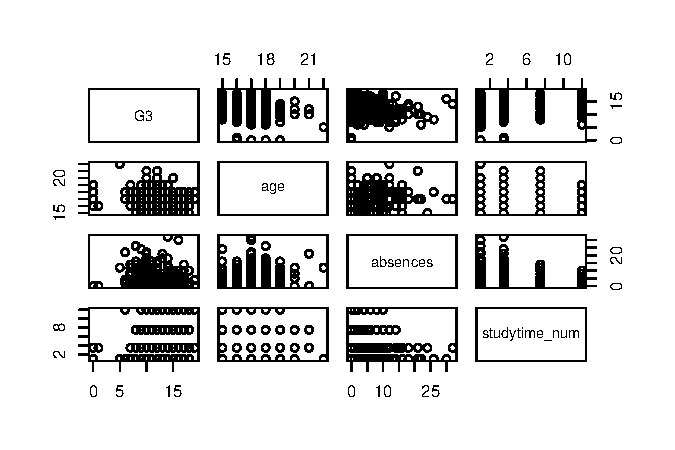
\includegraphics{Report_3-003}



From the pairs plot, we see that there is some linear correlation between absences and weekly study time. The correlation coefficient is -0.11, so the correlation is not very strong. We can also see some correlation between weekly time spent studying and final grade, G3. The correlation coefficient is a little higher, at 0.24, yet still relatively weak. Thus, we will not worry too much about multicolinearity.

From the pairs plot, we also observe that the bulk of the observations in the age variable are between ages 15 and 19. Thus, we group all the students who are older than 19 years old together. Additionally, we can also see that there are some outliers within the absences variable. We filter students who have had more than 30 absences. By constricting our data in this way, we also constrict the population we can generalize to. 


Notice also that four ordinal variables have a very small number of observations for some of their categories. Number of failures has only 13 observations for 2 and 3 failures each. Thus, we will to lump these categories together. Quality of family relationships, numbered 1-5, with 1 being very bad and 5 being excellent has only 21 and 29 observations for categories 1 and 2. Thus, we will lump categories 1 and 2 together. We will also lump categories 4 and 5 to balance the range of values that variable categories cover for this variable. Thus, category 1 now represents "bad family relationships," category 2 represents "okay family relationships," and category 3 represents "good family relationships." We do the same for the nominal variables workday alcohol consumption, Dalc.For home to school travel time, the categories are as follows: 1 - <15 min., 2 - 15 to 30 min., 3 - 30 min. to 1 hour, or 4 - >1 hour. Category 4 has only 16 observations. Thus, we combine it with category 3 so that category 3 now represents "more than ">30 minutes of travel time."




\section{MODEL BUILDING}
Build a training and a test dataset
\begin{Schunk}
\begin{Sinput}
> set.seed(47)
> require(leaps)
> col.subset <- sample(c(TRUE, FALSE), nrow(student_por_n), replace=TRUE, prob=c(1/3,2/3))
> col.tst <- student_por_n[col.subset,]
> col.trn <-student_por_n[!col.subset,]
\end{Sinput}
\end{Schunk}

Backwards Selection


Backward Selection Model at $\alpha = 0.05$
\begin{Schunk}
\begin{Sinput}
> bkwdselec <- lm(G3~school + sex + Mjob + failures + higher + famrel + Dalc + health, data=col.trn)
> summary(bkwdselec)
\end{Sinput}
\begin{Soutput}
Call:
lm(formula = G3 ~ school + sex + Mjob + failures + higher + famrel + 
    Dalc + health, data = col.trn)

Residuals:
     Min       1Q   Median       3Q      Max 
-11.3921  -1.5330   0.1508   1.4764   6.7290 

Coefficients:
             Estimate Std. Error t value Pr(>|t|)    
(Intercept)  11.69661    0.87636  13.347  < 2e-16 ***
schoolMS     -1.21907    0.29848  -4.084 5.38e-05 ***
sexM         -1.05286    0.28460  -3.699 0.000247 ***
Mjobhealth    0.95806    0.60334   1.588 0.113122    
Mjobother     0.14637    0.37125   0.394 0.693601    
Mjobservices  0.77540    0.44778   1.732 0.084132 .  
Mjobteacher   1.57507    0.51093   3.083 0.002198 ** 
failures     -2.27523    0.30600  -7.435 6.77e-13 ***
higheryes     1.33211    0.46722   2.851 0.004590 ** 
famrel        0.54980    0.21900   2.510 0.012464 *  
Dalc         -0.59288    0.28346  -2.092 0.037129 *  
health       -0.28378    0.09483  -2.993 0.002944 ** 
---
Signif. codes:  0 ‘***’ 0.001 ‘**’ 0.01 ‘*’ 0.05 ‘.’ 0.1 ‘ ’ 1

Residual standard error: 2.686 on 387 degrees of freedom
Multiple R-squared:  0.3507,	Adjusted R-squared:  0.3322 
F-statistic:    19 on 11 and 387 DF,  p-value: < 2.2e-16
\end{Soutput}
\end{Schunk}

Forwards Selection

Forwards Selection Model with $\alpha$-to-enter of 0.05. 

\begin{Schunk}
\begin{Sinput}
> fwdselec <- lm(G3~failures+school+sex+higher+health+famrel+Mjob+Dalc, data=col.trn)
> summary(fwdselec)
\end{Sinput}
\begin{Soutput}
Call:
lm(formula = G3 ~ failures + school + sex + higher + health + 
    famrel + Mjob + Dalc, data = col.trn)

Residuals:
     Min       1Q   Median       3Q      Max 
-11.3921  -1.5330   0.1508   1.4764   6.7290 

Coefficients:
             Estimate Std. Error t value Pr(>|t|)    
(Intercept)  11.69661    0.87636  13.347  < 2e-16 ***
failures     -2.27523    0.30600  -7.435 6.77e-13 ***
schoolMS     -1.21907    0.29848  -4.084 5.38e-05 ***
sexM         -1.05286    0.28460  -3.699 0.000247 ***
higheryes     1.33211    0.46722   2.851 0.004590 ** 
health       -0.28378    0.09483  -2.993 0.002944 ** 
famrel        0.54980    0.21900   2.510 0.012464 *  
Mjobhealth    0.95806    0.60334   1.588 0.113122    
Mjobother     0.14637    0.37125   0.394 0.693601    
Mjobservices  0.77540    0.44778   1.732 0.084132 .  
Mjobteacher   1.57507    0.51093   3.083 0.002198 ** 
Dalc         -0.59288    0.28346  -2.092 0.037129 *  
---
Signif. codes:  0 ‘***’ 0.001 ‘**’ 0.01 ‘*’ 0.05 ‘.’ 0.1 ‘ ’ 1

Residual standard error: 2.686 on 387 degrees of freedom
Multiple R-squared:  0.3507,	Adjusted R-squared:  0.3322 
F-statistic:    19 on 11 and 387 DF,  p-value: < 2.2e-16
\end{Soutput}
\end{Schunk}

This is the same as our backwards selection model! From here on out, we will be working with the model "fwdselec".


\textbf{Interaction}

\begin{Schunk}
\begin{Sinput}
> ggplot(data = col.trn, aes(x= Dalc, y=G3, color=higher)) + geom_smooth(method='lm',formula=y~x)
> inter <- lm(G3 ~ higher*Dalc,data = col.trn)
> summary(inter)
\end{Sinput}
\begin{Soutput}
Call:
lm(formula = G3 ~ higher * Dalc, data = col.trn)

Residuals:
     Min       1Q   Median       3Q      Max 
-12.4286  -1.4286   0.1579   1.5714   7.1564 

Coefficients:
               Estimate Std. Error t value Pr(>|t|)    
(Intercept)      8.5000     1.0325   8.233 2.70e-15 ***
higheryes        5.5137     1.1209   4.919 1.28e-06 ***
Dalc             0.3421     0.6946   0.492   0.6226    
higheryes:Dalc  -1.9272     0.7786  -2.475   0.0137 *  
---
Signif. codes:  0 ‘***’ 0.001 ‘**’ 0.01 ‘*’ 0.05 ‘.’ 0.1 ‘ ’ 1

Residual standard error: 3.063 on 395 degrees of freedom
Multiple R-squared:  0.1382,	Adjusted R-squared:  0.1316 
F-statistic: 21.11 on 3 and 395 DF,  p-value: 1.051e-12
\end{Soutput}
\end{Schunk}

We looked at all the possible interaction terms and the only significant one at the 0.05 value was between workday alcohol consumption, Dalc, and whether or not a student wants to go to higher education. The interaction does not make sense within the context of this problem, so we will omitt it from the model. 

Additionally, based on the VIF values for our model, we do not have a multicolinearity problem. 
\begin{Schunk}
\begin{Sinput}
> require(car)
> vif(fwdselec)
\end{Sinput}
\begin{Soutput}
             GVIF Df GVIF^(1/(2*Df))
failures 1.121600  1        1.059056
school   1.143255  1        1.069231
sex      1.095476  1        1.046650
higher   1.160920  1        1.077460
health   1.043789  1        1.021660
famrel   1.045958  1        1.022721
Mjob     1.225436  4        1.025738
Dalc     1.073840  1        1.036263
\end{Soutput}
\end{Schunk}


\section{MODEL SELECTION}

Now we will compare our model with a nested model with two fewer variables.


Nested F-Tests
\begin{Schunk}
\begin{Sinput}
> summary(fwdselec)
\end{Sinput}
\begin{Soutput}
Call:
lm(formula = G3 ~ failures + school + sex + higher + health + 
    famrel + Mjob + Dalc, data = col.trn)

Residuals:
     Min       1Q   Median       3Q      Max 
-11.3921  -1.5330   0.1508   1.4764   6.7290 

Coefficients:
             Estimate Std. Error t value Pr(>|t|)    
(Intercept)  11.69661    0.87636  13.347  < 2e-16 ***
failures     -2.27523    0.30600  -7.435 6.77e-13 ***
schoolMS     -1.21907    0.29848  -4.084 5.38e-05 ***
sexM         -1.05286    0.28460  -3.699 0.000247 ***
higheryes     1.33211    0.46722   2.851 0.004590 ** 
health       -0.28378    0.09483  -2.993 0.002944 ** 
famrel        0.54980    0.21900   2.510 0.012464 *  
Mjobhealth    0.95806    0.60334   1.588 0.113122    
Mjobother     0.14637    0.37125   0.394 0.693601    
Mjobservices  0.77540    0.44778   1.732 0.084132 .  
Mjobteacher   1.57507    0.51093   3.083 0.002198 ** 
Dalc         -0.59288    0.28346  -2.092 0.037129 *  
---
Signif. codes:  0 ‘***’ 0.001 ‘**’ 0.01 ‘*’ 0.05 ‘.’ 0.1 ‘ ’ 1

Residual standard error: 2.686 on 387 degrees of freedom
Multiple R-squared:  0.3507,	Adjusted R-squared:  0.3322 
F-statistic:    19 on 11 and 387 DF,  p-value: < 2.2e-16
\end{Soutput}
\begin{Sinput}
> #delete dalc and famrel (least significant)
> fwdselec_reduced <- lm(G3 ~ failures + school + sex + higher + health + Mjob, data=col.trn)
\end{Sinput}
\end{Schunk}

"Dalc" and "famrel" are the least significant of those included in our model. Thus, we will omit them to generate a nested model with two fewer variables than the original. We will now test the hypothesis that both "Dalc" and "famrel" are not needed in the model - $H_{0}=\beta_{Dalc}=\beta_{famrel}=0$ - using a nested F-test. 

\begin{Schunk}
\begin{Sinput}
> #compare each with anova
> anova(fwdselec, fwdselec_reduced)
\end{Sinput}
\begin{Soutput}
Analysis of Variance Table

Model 1: G3 ~ failures + school + sex + higher + health + famrel + Mjob + 
    Dalc
Model 2: G3 ~ failures + school + sex + higher + health + Mjob
  Res.Df    RSS Df Sum of Sq      F   Pr(>F)   
1    387 2791.9                                
2    389 2869.0 -2   -77.103 5.3439 0.005136 **
---
Signif. codes:  0 ‘***’ 0.001 ‘**’ 0.01 ‘*’ 0.05 ‘.’ 0.1 ‘ ’ 1
\end{Soutput}
\end{Schunk}

We get a p-value of 0.0087, indicating, at the $\alpha=0.05$ level, that we can rejec the null hypothesis. Indeed, "Dalc" and/or "famrel" are needed in the model. Let's take a quick look at the significance of the variables in the reduced model.

\begin{Schunk}
\begin{Sinput}
> summary(fwdselec_reduced)
\end{Sinput}
\begin{Soutput}
Call:
lm(formula = G3 ~ failures + school + sex + higher + health + 
    Mjob, data = col.trn)

Residuals:
    Min      1Q  Median      3Q     Max 
-11.395  -1.493  -0.023   1.701   6.605 

Coefficients:
             Estimate Std. Error t value Pr(>|t|)    
(Intercept)   12.3425     0.6345  19.452  < 2e-16 ***
failures      -2.4385     0.3053  -7.988 1.56e-14 ***
schoolMS      -1.2776     0.3008  -4.248 2.71e-05 ***
sexM          -1.1187     0.2822  -3.964 8.77e-05 ***
higheryes      1.4386     0.4713   3.053  0.00242 ** 
health        -0.2527     0.0951  -2.657  0.00820 ** 
Mjobhealth     0.9377     0.6083   1.541  0.12401    
Mjobother      0.1551     0.3754   0.413  0.67968    
Mjobservices   0.7528     0.4527   1.663  0.09709 .  
Mjobteacher    1.5620     0.5164   3.024  0.00266 ** 
---
Signif. codes:  0 ‘***’ 0.001 ‘**’ 0.01 ‘*’ 0.05 ‘.’ 0.1 ‘ ’ 1

Residual standard error: 2.716 on 389 degrees of freedom
Multiple R-squared:  0.3328,	Adjusted R-squared:  0.3173 
F-statistic: 21.56 on 9 and 389 DF,  p-value: < 2.2e-16
\end{Soutput}
\end{Schunk}

Interesting - "higheryes" has become significant at the 0.001 level, whereas it was not in the full model. This would indicate collinearity. That said, its significance only very slightly increased. Let's continue working with the full model.

\section{MODEL INTERPRETATION AND FIT}


$$E[Y]=12.27-1.98X_{failures}-1.31X_{schoolMS}-1.10X_{sexM}+1.55X_{higheryes}-0.26X_{health}$$
$$+0.85X_{Mjobhealth}+0.08X_{Mjobother}+0.70X_{Mjobservices}+1.53X_{Mjobteacher} $$

\section{SUMMARY}

\end{document}
